

\subsection{Bohrsches Atommodell: klassisch-quantisierte Bahnen}
\index{Bohrsches Atommodell}
\index{Quantisierung}
\index{Elektronenbahn}
\index{Wasserstoffatom}
\index{Energieniveau}
\index{Spektrallinie}

Das rutherfordsche Kernmodell zeigte, dass das Atom aus einem kleinen,
positiv geladenen Kern und einer Elektronenhülle besteht. Damit war die
räumliche Struktur des Atoms wesentlich besser verstanden als im
thomsonschen Modell. Ein entscheidendes Problem blieb jedoch ungelöst:
Nach der klassischen Elektrodynamik wäre ein Atom mit umlaufenden
Elektronen nicht stabil.

Ein Elektron, das sich auf einer Kreisbahn um den Atomkern bewegt, ist
ständig beschleunigt. Nach der klassischen Theorie müsste ein beschleunigtes
geladenes Teilchen elektromagnetische Strahlung aussenden. Dadurch würde das
Elektron Energie verlieren. Seine Bahn würde kleiner werden, und es müsste
schließlich in den Kern stürzen. Klassisch betrachtet wäre das Atom also
instabil.

Niels Bohr löste dieses Problem nicht durch eine vollständig neue Mechanik,
sondern durch zusätzliche Annahmen. Er verband das rutherfordsche Kernmodell
mit der Idee der Quantisierung. Das Elektron durfte sich nicht auf beliebigen
Bahnen bewegen, sondern nur auf bestimmten erlaubten Bahnen. Auf diesen Bahnen
strahlt es keine Energie ab.

Die erste zentrale Annahme lautet daher:

\[
\text{Elektronen können sich nur auf bestimmten stationären Bahnen bewegen.}
\]

Jede dieser Bahnen besitzt eine bestimmte Energie. Solange sich das Elektron
auf einer solchen stationären Bahn befindet, bleibt seine Energie konstant.
Ein Energieverlust durch kontinuierliche Strahlung findet in diesem Modell
nicht statt.

Die zweite zentrale Annahme betrifft Übergänge zwischen diesen Bahnen. Ein
Elektron kann von einer Bahn mit höherer Energie auf eine Bahn mit niedrigerer
Energie wechseln. Dabei wird ein Photon ausgesendet. Die Energie dieses Photons
entspricht genau der Energiedifferenz zwischen beiden Bahnen:

\[
\Delta E = E_2 - E_1 = h f
\]

Hierbei ist \(h\) das plancksche Wirkungsquantum und \(f\) die Frequenz des
ausgesendeten Lichts. Damit verknüpfte Bohr das Atommodell direkt mit der
Quantentheorie des Lichts.
\FloatBarrier
\begin{figure}[H]
	\centering
	 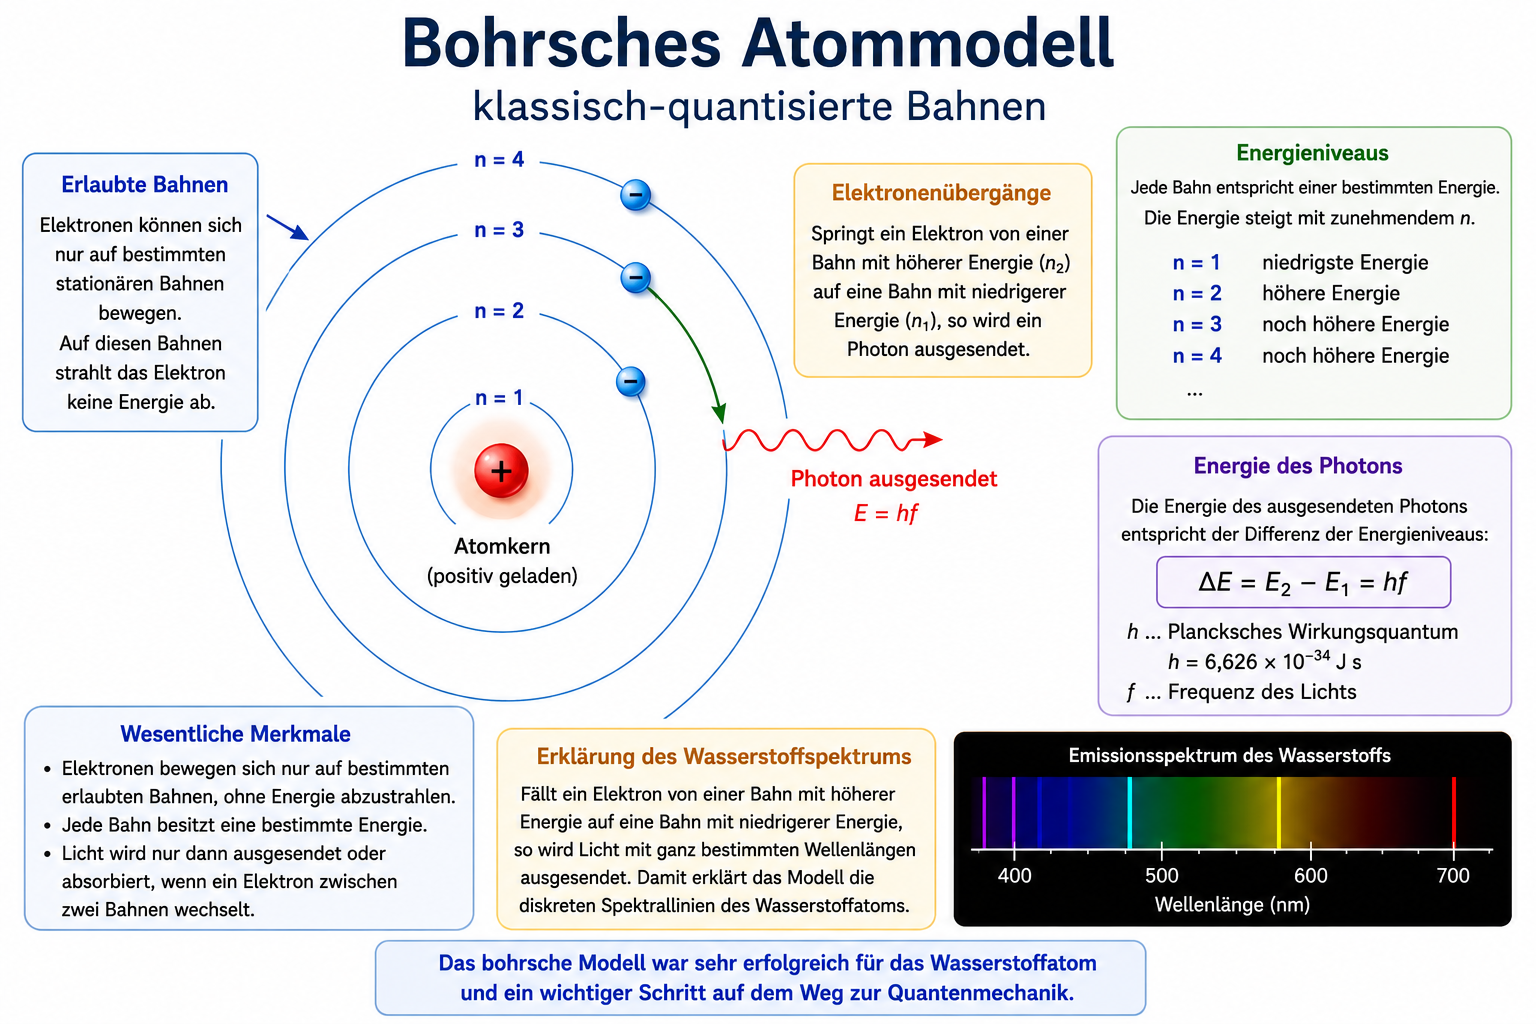
\includegraphics[width=0.75\textwidth]{bilder/bohr_atommodell}
	\caption{Schematische Darstellung des bohrschen Atommodells. Das Elektron
		bewegt sich nur auf bestimmten erlaubten Bahnen. Beim Übergang auf eine
		niedrigere Bahn wird ein Photon mit der Energie \(\Delta E = hf\)
		ausgesendet.}
	\label{fig:bohrsches_atommodell}
\end{figure}

Besonders erfolgreich war das bohrsche Atommodell beim Wasserstoffatom. Dieses
besteht aus einem Proton als Kern und einem einzigen Elektron. Für dieses
einfache System konnte Bohr die diskreten Spektrallinien des Wasserstoffs
erklären. Das war ein großer Fortschritt, denn diese Spektrallinien waren
experimentell längst bekannt, aber klassisch nicht verständlich.

Die erlaubten Bahnen entsprechen im bohrschen Modell bestimmten Energieniveaus.
Wechselt das Elektron zwischen zwei Energieniveaus, entsteht Licht mit einer
bestimmten Frequenz. Deshalb sendet ein Atom nicht beliebige Farben aus,
sondern nur bestimmte Spektrallinien.

Für das Elektron bedeutete Bohrs Modell eine neue physikalische Rolle. Es war
nicht mehr einfach ein klassisches Teilchen, das auf beliebigen Bahnen um den
Kern kreist. Seine Bewegung war durch Quantisierungsbedingungen eingeschränkt.
Das Elektron wurde damit zum Träger diskreter Energiezustände im Atom.

Trotz seines Erfolges blieb das bohrsche Modell ein Zwischenmodell. Es arbeitete
noch mit anschaulichen Elektronenbahnen, führte aber gleichzeitig künstliche
Quantisierungsregeln ein. Es erklärte das Wasserstoffatom gut, versagte aber
bei Atomen mit mehreren Elektronen und bei feineren Details der Spektren.

Der eigentliche Wert des bohrschen Modells liegt deshalb in seiner Übergangsrolle.
Es zeigte, dass die Stabilität der Atome und ihre Spektrallinien nur durch
Quantisierung verstanden werden können. Damit führte es direkt weiter zur
modernen Quantenmechanik, in der Elektronen nicht mehr als kleine Teilchen auf
festen Bahnen beschrieben werden, sondern durch Wellenfunktionen und
Aufenthaltswahrscheinlichkeiten.

\index{Bohrsches Atommodell}
\index{Elektronenbahn}
\index{Stationäre Bahn}
\index{Energieniveau}
\index{Spektrallinie}
\index{Wasserstoffatom}




\begin{MathBox}[Bohrs Quantisierungsbedingung]
	
	\label{box:bohr-drehimpulsquantisierung}
	Im bohrschen Atommodell ist der Drehimpuls des Elektrons nicht beliebig,
	sondern quantisiert:
	
	\[
	L = m_\mathrm{e} v r = n \hbar ,
	\qquad n = 1,2,3,\ldots
	\]
	
	Die ganze Zahl \(n\) heißt Hauptquantenzahl. Sie bestimmt im einfachen
	bohrschen Modell das Energieniveau des Elektrons.
	
\end{MathBox}